\section{Proposed Designs}
Our design aims to retain the high energy efficiency potential demonstrated in Section~2, while integrating the urban constraints discussed in Section~3 and the user requirements outlined in Section~4. The result is a narrow, lightweight, enclosed vehicle assimilated to a cycle.

\textbf{1. Efficiency:}  
By minimizing mass and frontal area, using low rolling resistance wheels, and optimizing aerodynamics (target $C_d \approx 0.15$), the proposed vehicle matches the energy performance of state-of-the-art velomobiles and outperforms an electric car and an ICE car by a factor 10 and 50 respectively on an efficiency level.

\textbf{2. Human experience:}  
Unlike velomobiles or e-bikes, this concept improves rider visibility and perceived safety by raising the riding position without compromising stability, thanks to a leaning mechanism. This system also simplifies ingress and egress (the vehicle tilts forward to assist the user) and allows for vertical parking, improving usability in dense urban settings.

\textbf{3. Urban compatibility:}  
The vehicle occupies far less road and parking space than a car, and remains legally within bicycle limits, allowing access to bike lanes while being able to keep up with traffic pace.

\vspace{0.3em}

Although existing solutions will be examined in more detail further, we can already see that :  \\
\textbf{E-bikes and velomobiles} often come short from a user standpoint as they fail to address minimal comfort and safety requirement.
While \textbf{Cars}, on the other hand, fail on efficiency and urban integration by being oversized in both energy and space usage.

Here are presented the two main parameters of the design space that we will study on a dynamic standpoint : the choice between a three or four-wheel configuration (figure \ref{fig:number_of_wheel}), and two leaning mechanisms (figure \ref{fig:leaning_mechanism}) that use either pivot arm vs. linear-guided suspension to ensure stability while enabling an elevated riding position. 

Figure \ref{fig:vertical_parking_easy_egress} highlight how the proposed layout benefit egress/ingress and vertical storage by allowing to recline the seat and let the user easily redress the vehicle.


\begin{figure}[h!]
    \centering
    \begin{minipage}{0.45\linewidth}
        \centering
        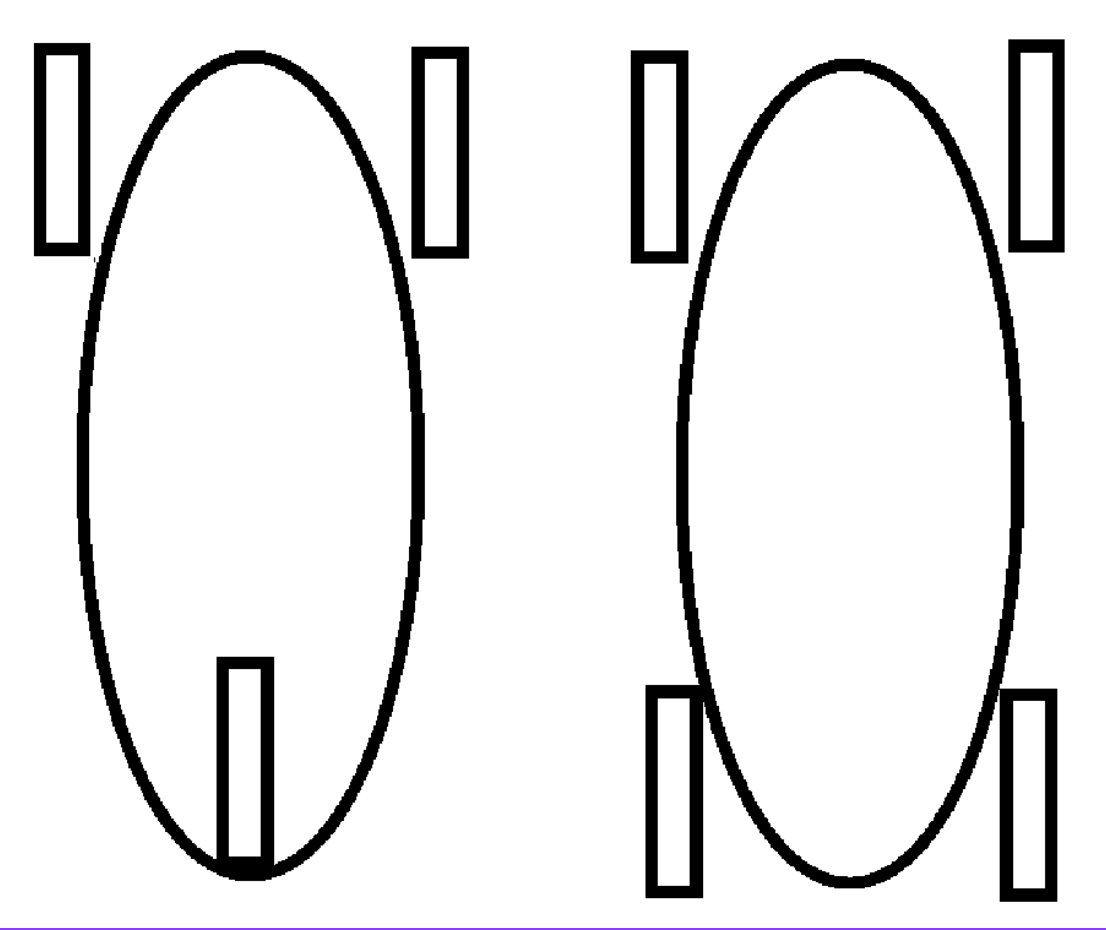
\includegraphics[width=\linewidth]{Figures/ch4_three_vs_four_wheel.png}
        \caption{Three and Four wheeler configuration}
        \label{fig:number_of_wheel}
    \end{minipage}
    \hfill
    \begin{minipage}{0.35\linewidth}
        \centering
        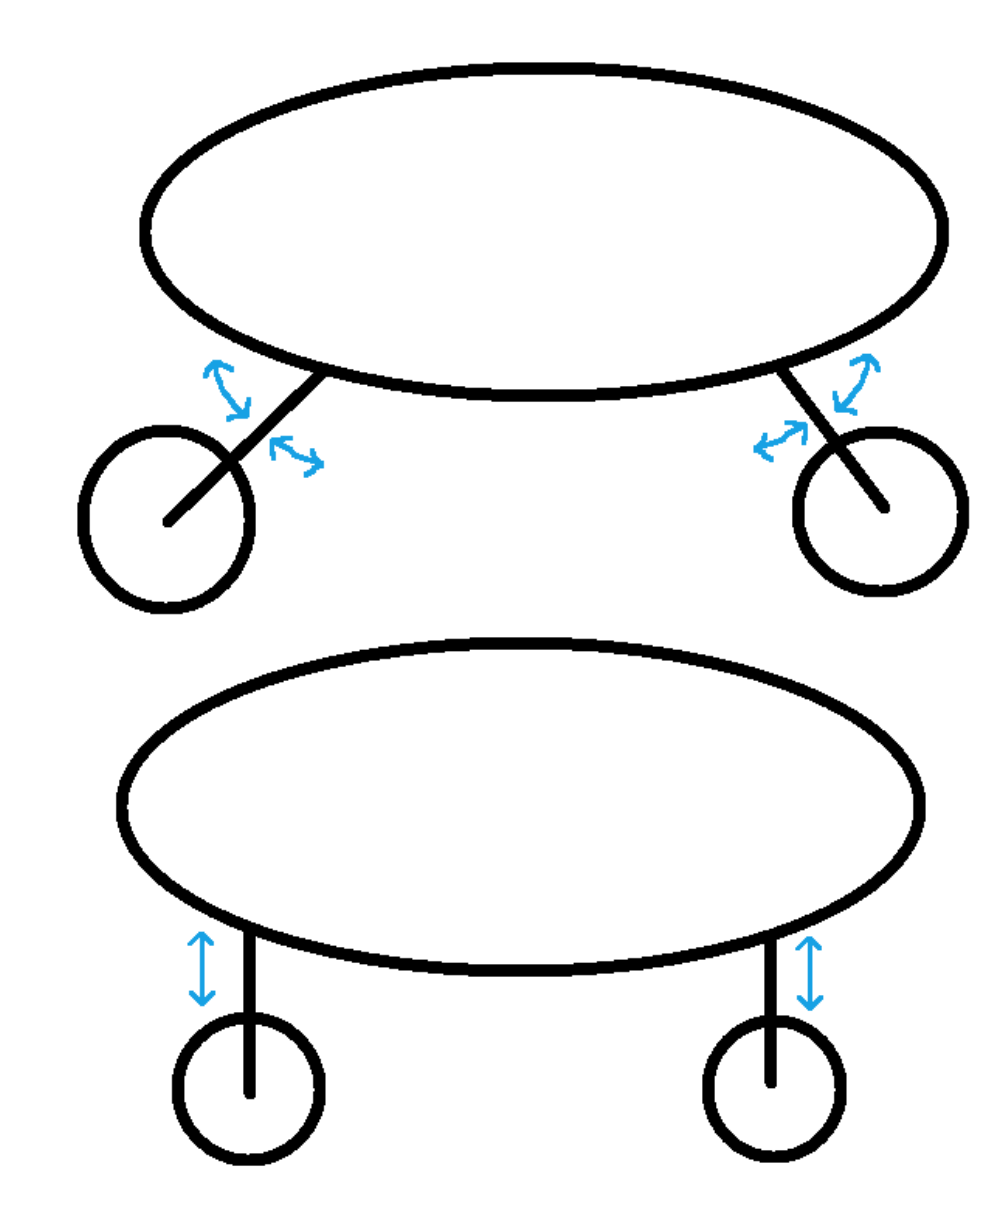
\includegraphics[width=\linewidth]{Figures/ch4_WheelMechanismHeightAdaption.png}
        \caption{Leaning mechanism based either on a pivot or a linear-guided suspension}
        \label{fig:leaning_mechanism}
    \end{minipage}
\end{figure}

\newpage 

\begin{figure}[h!]
    \centering
    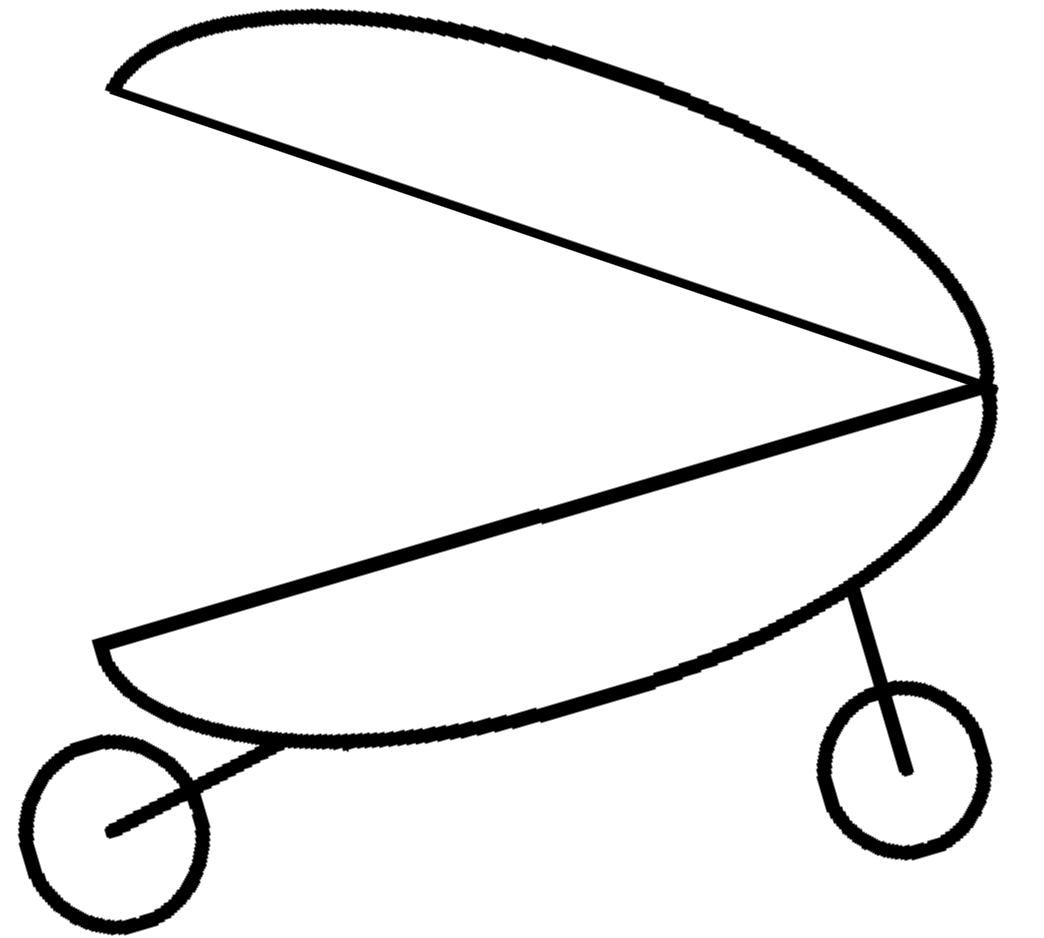
\includegraphics[width=0.5\linewidth]{Figures/ch4_EgressReclining.png}
    \caption{Simplified Egress and vertical parking}
    \label{fig:vertical_parking_easy_egress}
\end{figure}

\vfill


\subsection{Comparative Evaluation}
The proposed design consistently scores higher across efficiency, urban integration, and human experience compared to both cars and cycle-based alternatives. By combining a compact footprint with enhanced protection and usability, it bridges the gap between comfort and sustainability. However, this performance comes at the cost of increased mechanical and control complexity, inherent to narrow-track vehicles. To address these challenges, we will evaluate multiple mechanical configurations including three-wheel and four-wheel variants, as well as different leaning actuation strategies based on linear actuators or pivot mechanisms. These configurations will be analyzed both from a static standpoint to assess tipping stability and from a dynamic perspective. The following chapters will dive into these aspects, starting with the analysis of static behavior before transitioning to the more demanding problem of dynamic stabilization and control.

\newpage 

\begin{table}[h!]
\caption{Performance Comparison}
\centering
\renewcommand{\arraystretch}{1.25}
\setlength{\tabcolsep}{5pt}
\begin{tabularx}{\textwidth}{lXXXXX}
\toprule
\textbf{Parameter} & \textbf{E-Bike} & \textbf{Velomobile} & \textbf{ ICE Car} & \textbf{Electric Car} & \textbf{Proposed Design} \\
\midrule
\multicolumn{6}{l}{\textbf{Section 1: Efficiency}} \\
Drive train efficiency        & \cellcolor{LightGreen}$\geq70\%$     & \cellcolor{LightGreen}$\geq70\%$     & \cellcolor{LightRed}$\leq30\%$       & \cellcolor{LightGreen}$\geq80\%$     & \cellcolor{LightGreen}$\geq80\%$ \\
$C_d$ (drag coefficient)      & \cellcolor{LightRed}1                & \cellcolor{LightGreen}0.15           & \cellcolor{LightRed}0.3              & \cellcolor{LightOrange}0.2           & \cellcolor{LightGreen}0.15 \\
Frontal area (m²)            & \cellcolor{LightGreen}0.5            & \cellcolor{LightGreen}0.35           & \cellcolor{LightRed}2.3              & \cellcolor{LightRed}2.3              & \cellcolor{LightGreen}$\leq$0.7 \\
Mass $m$ (kg)                & \cellcolor{LightGreen}85             & \cellcolor{LightGreen}110            & \cellcolor{LightRed}1100             & \cellcolor{LightRed}1300             & \cellcolor{LightGreen}$<$250 \\
$C_{rr}$ (rolling resistance) & \cellcolor{LightGreen}0.004          & \cellcolor{LightGreen}0.004          & \cellcolor{LightOrange}0.01          & \cellcolor{LightOrange}0.01          & \cellcolor{LightGreen}0.004 \\
\midrule
\multicolumn{6}{l}{\textbf{Section 2: Urban Elements}} \\
Width (cm)                  & \cellcolor{LightGreen}50             & \cellcolor{LightGreen}70             & \cellcolor{LightRed}180              & \cellcolor{LightRed}180              & \cellcolor{LightGreen}$<$70 \\
Parking space (m²)          & \cellcolor{LightGreen}1              & \cellcolor{LightGreen}1.5            & \cellcolor{LightRed}12               & \cellcolor{LightRed}12               & \cellcolor{LightGreen}$\approx$0.7 \\
Speed (km/h)                & \cellcolor{LightOrange}45            & \cellcolor{LightOrange}45            & \cellcolor{LightGreen}120            & \cellcolor{LightGreen}120            & \cellcolor{LightGreen}60-80 \\
Power-to-weight (continuous) & \cellcolor{LightOrange}13 W/kg       & \cellcolor{LightOrange}10 W/kg       & \cellcolor{LightGreen}50 W/kg        & \cellcolor{LightGreen}60 W/kg        & \cellcolor{LightOrange}$1–25 W/kg^*$ \\
Power-to-weight (peak)       & \cellcolor{LightOrange}16 W/kg       & \cellcolor{LightOrange}13 W/kg       & \cellcolor{LightGreen}50 W/kg        & \cellcolor{LightGreen}120 W/kg       & \cellcolor{LightGreen}60 W/kg \\
\midrule
\multicolumn{6}{l}{\textbf{Section 3: Human Elements}} \\
Feeling visible / high road   & \cellcolor{LightGreen}Good           & \cellcolor{LightRed}Bad              & \cellcolor{LightGreen}Good           & \cellcolor{LightGreen}Good           & \cellcolor{LightGreen}Good \\
Feeling protected             & \cellcolor{LightRed}Poor             & \cellcolor{LightOrange}Fair          & \cellcolor{LightGreen}Good           & \cellcolor{LightGreen}Good           & \cellcolor{LightGreen}Good \\
Physical effort               & \cellcolor{LightOrange}Medium        & \cellcolor{LightOrange}Medium        & \cellcolor{LightGreen}None           & \cellcolor{LightGreen}None           & \cellcolor{LightGreen}minimal \& Constant \\
Cargo \& passenger capacity   & \cellcolor{LightRed}Low              & \cellcolor{LightOrange}Fair          & \cellcolor{LightGreen}Good           & \cellcolor{LightGreen}Good           & \cellcolor{LightGreen}2 adult or 4-5 bag \\
Weather / thermal protection  & \cellcolor{LightRed}Minimal          & \cellcolor{LightGreen}Good           & \cellcolor{LightGreen}Good           & \cellcolor{LightGreen}Good           & \cellcolor{LightGreen}Good \\
Privacy / comfort             & \cellcolor{LightRed}Poor             & \cellcolor{LightOrange}Fair          & \cellcolor{LightGreen}Good           & \cellcolor{LightGreen}Good           & \cellcolor{LightGreen}Good \\
Ease of entry / exit          & \cellcolor{LightOrange}Fair          & \cellcolor{LightRed}Difficult        & \cellcolor{LightGreen}Good           & \cellcolor{LightGreen}Good           & \cellcolor{LightGreen}Front-tilt, upright \\
\bottomrule
\end{tabularx}
\end{table}

\paragraph*{Note on Power-to-Weight Ratio ($^*$):}
The continuous power-to-weight ratio marked with an asterisk refers to the average sustained power a person can provide typically around \textbf{1\,W/kg}. This estimate is sufficient for flat terrain and steady-state cruising, where only aerodynamic and rolling resistance need to be overcome.

While slope climbing and acceleration phases require much higher instantaneous power, up to \textbf{25\,W/kg}. The energy spent climbing is largely recovered when descending. As a result, over the course of a typical ride, elevation changes and accelerations tend to cancel out in terms of net energy expenditure assuming the losses are compensated. 

Therefore, even though higher peak power is occasionally needed, a continuous input of \textbf{1\,W/kg} is generally enough to sustain average cruising performance effectively allowing the user to achieve what would otherwise require a \textbf{25\,W/kg} system, provided that energy buffering (e.g., a battery or gravity) absorbs the transient demands.
